\chapter{总结与展望}
% //TODO: add something

\section{论文总结}

\section{工作展望}
在技术实现上,构建了两个版本的量子线路转化为TDD的工具,分别基于C语言和Python语言。这些工具的开发对于实现我们的研究方法至关重要,提高了实验的灵活性和效率。
其中的C语言的TDD支持任意维度张量,例如对双比特CNOT门,既可以按图\ref{fig:cnot-4}中的张量维度为4,
即按照索引为$q_1,q_0$进行表示。也可以按图\ref{fig:cnot-2}中的张量维度为4,
即按照索引为$q_3,q_2,q_1,q_0$进行表示。这样的设计大大提高了TDD的表示能力,为更复杂系统的验证提供了基础。
\begin{figure}[!htbp]
    \centering
    \begin{subfigure}[b]{.4\textwidth}
        \centering
        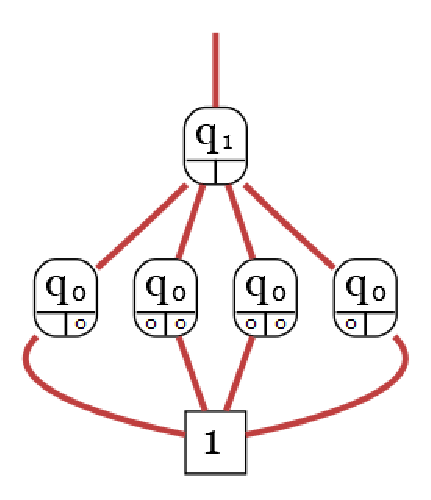
\includegraphics[height = 6cm]{Img/cnot.eps}
        \caption{张量维度为4的CNOT门的TDD表示}
        \label{fig:cnot-4}
    \end{subfigure}
    \begin{subfigure}[b]{.4\textwidth}
        \centering
        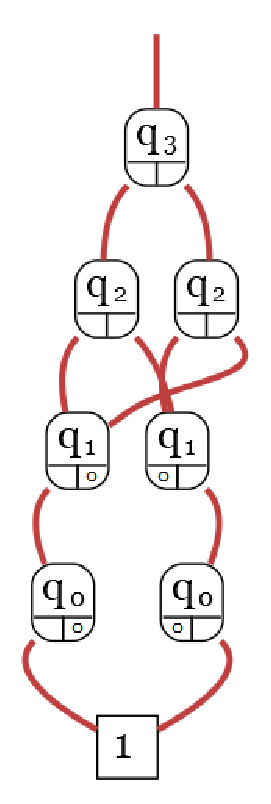
\includegraphics[height=6cm]{Img/cx.eps}
        \caption{张量维度为2的CNOT门的TDD表示}
        \label{fig:cnot-2}
    \end{subfigure}
    \caption{C语言版的TDD支持任意维度的例子}
    \label{fig-cnot}
\end{figure}
% //TODO: add limdd data
\subsection*{limdd的改进}
由于量子状态都在同一希尔伯特空间中。因此作用某些算子后,不同的量子状态可能等价。
当存储算子的资源少于存储状态的资源时,就有可能存储算子表示不同的状态\citep{vinkhuijzen2023limdd}。图\ref{fig:qmdd-example}表示了一个QMDD的例子,应用等价性,可以化简为图\ref{fig:limdd-example}。
TDD也可以应用类似技术,进行进一步化简,从而降低资源要求。
\begin{figure}[!htbp]
    \centering
    \begin{subfigure}[b]{.4\textwidth}
        \centering
        \includegraphics[height=8cm]{Img/limdd.pdf}
        \caption{一个QMDD示例}
        \label{fig:qmdd-example}
    \end{subfigure}
    \begin{subfigure}[b]{.4\textwidth}
        \centering
        \includegraphics[height=8cm]{Img/limdd_reduce.pdf}
        \caption{应用等价性化简图\ref{fig:qmdd-example}}
        \label{fig:limdd-example}
    \end{subfigure}
\end{figure}
% //TODO:add here
\textcolor{red}{limdd的原理}